\begin{figure}[h]
\centering
    \subfloat{
      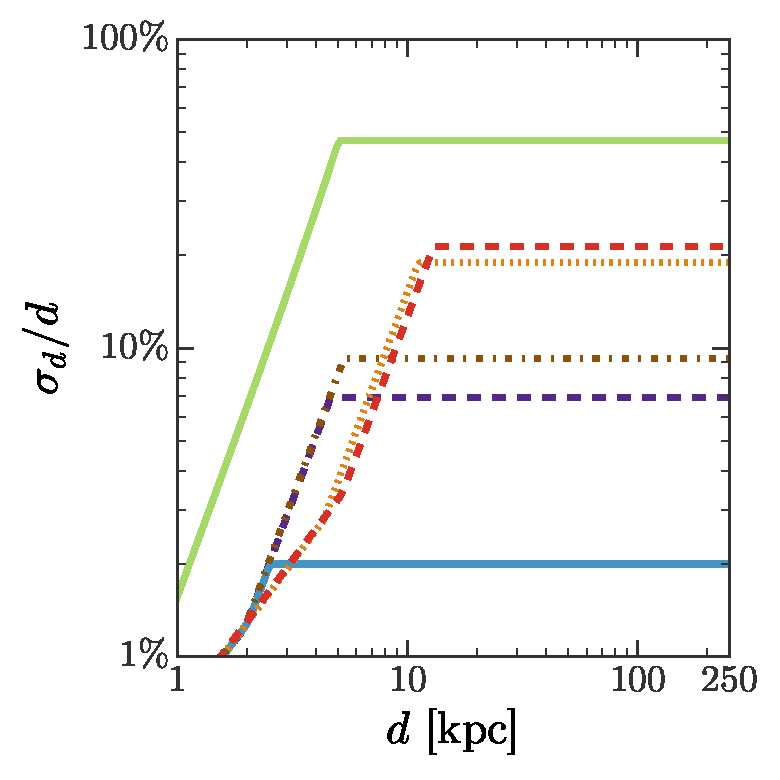
\includegraphics[width=0.48\textwidth]{figures/frac-plx-err.pdf}
    }
    \subfloat{
      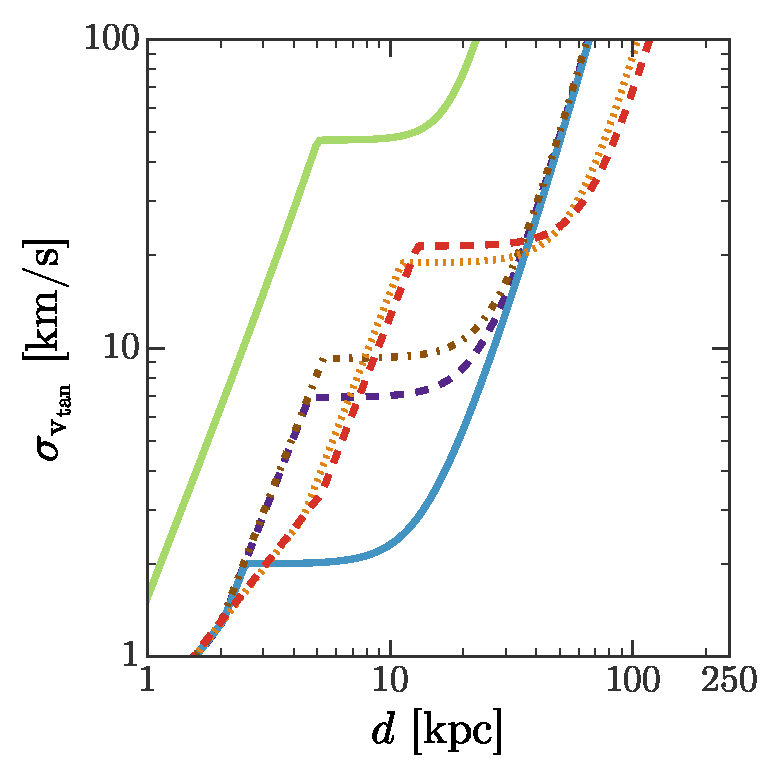
\includegraphics[width=0.48\textwidth]{figures/vtan-err.pdf}
    }
\caption{Estimates for the astrometric precision of the end-of-mission data
release from the \gaia\ mission for individual stars of different types.
\textit{Left}: Fractional parallax or distance uncertainty for different stellar
tracers as a function of distance. When the \gaia\ parallax uncertainty becomes
larger than the distance uncertainty for an alternate distance measurement
method, the minimum uncertainty is assumed. For example, for RR Lyrae (RRL)
stars, distance measurements from the period-luminosity relation are
$\approx$2\%. For other stars, photometric distance uncertainties range from
$\approx$8--50\%. \text{Right}: Tangential velocity uncertainty using the
fractional distance uncertainties in the left panel and the proper motion
uncertainties from \gaia\ for a star with a tangential velocity $v_{\rm tan} =
100~\kms$.}
\label{fig:gaia-tracer-errs}
\end{figure}